% Scalar instruction entry source: tools/generate_scalar_instruction_catalog.py.
\subsection{\texttt{FEXP}}
\label{sec:scalar-fexp}
\index{FEXP@\texttt{FEXP}}
\begin{sloppypar}\noindent\textbf{Purpose.} Computes the floating-point exponential of SrcL and writes the rounded result to RegDst.\end{sloppypar}\smallskip
\noindent\textbf{Syntax.}\par
\begin{lstlisting}[style=ptoscalarcode]
fexp.{T} SrcL, ->RegDst
\end{lstlisting}
\noindent\textbf{Encoding.}\par
\noindent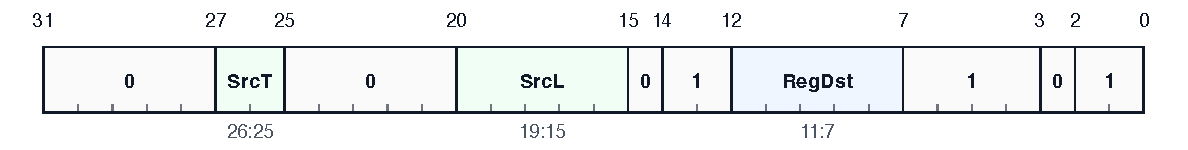
\includegraphics[width=\textwidth]{figs/encoding/scalar_instruction_entries/enc_fexp.pdf}\par\smallskip
\begin{description}[leftmargin=0.18\linewidth,style=nextline]
\item[Format] \texttt{L32} \texttt{32-bit} scalar word.
\item[Pattern] \texttt{00000..00000.....011.....1111011}.
\end{description}
\noindent\textbf{Classification.}\par
\begin{description}[leftmargin=0.18\linewidth,style=nextline]
\item[Category] Floating-Point and Conversion.
\item[Family] Floating-point Arithmetic.
\item[Execution class] \texttt{FSU}; uop\_kind=FSU.
\end{description}
\noindent\textbf{Operand fields.}\par
\begin{description}[leftmargin=0.18\linewidth,style=nextline]
\item[\texttt{RegDst}] Bits \texttt{11:7 (5b)}. 5-bit scalar destination register that receives the floating-point, conversion, or FP-compare result encoded in scalar register storage; X0 discards the write.
\item[\texttt{SrcL}] Bits \texttt{19:15 (5b)}. 5-bit scalar source register holding the left or only floating-point/conversion operand; SrcType or the assembly suffix determines the interpreted format.
\item[\texttt{SrcType}] Bits \texttt{26:25 (2b)}. 2-bit source format selector for floating-point or conversion operands. The assembly suffix \{T\} names the selected floating-point element format.
\end{description}
\noindent\textbf{Operation.}\par
\begin{lstlisting}[style=ptoscalarcode]
value = FPRead(SrcL, T)
Write(RegDst, FPRound(exp(value), T))
\end{lstlisting}
\Needspace{0.08\textheight}
